%# -*- coding: utf-8-unix -*-
%%==================================================
%% chapter01.tex for SJTU Master Thesis
%%==================================================

%\bibliographystyle{sjtu2}%[此处用于每章都生产参考文献]
\chapter{系统实验与验证}
\label{chap:experiment}
在第\ref{chap:systemdesign}章,我们介绍了DOBBS系统的架构设计和两个重要的概念。第\ref{chap:systemimpl}章,我们在系统设计的基础上介绍了系统
各个模块的实现。本章则在前两章基础上,对整个系统进行了验证。

\section{实验环境配置和搭建}
在本论文的实验部分需要构造的主要有三部分,一是Ceph集群,二是Monitor集群和Center节点,三则是Client。在本实验中,我们采用了4台服务器作为OSD搭载的机器,
而Ceph集群需要一个Ceph监控器,所以我们用一台专用的服务器表示Ceph监控器。因此,我们一共使用五台服务器构建Ceph集群。这五台服务器都是HP Compaq Pro 6300
Microtower,他们的CPU是Intel Core i3-3220 3.30GHz,内存是4G DDR3 SDRAM。其上的操作系统是Ubuntu 14.04.5内核是Linux kernel的4.4.0-31-generic版本。
其中四台服务器作为OSD搭载服务器,有两台搭载SSD,两台搭载HDD。SSD是120GB KINGSTON V300 SATA3 SSD,HDD是1TB Seagate 520S SATA HDD。一共有四块SSD,四块HDD,
搭载SSD的机器各有两块SSD,搭载HDD的机器各有两块HDD,我们一共有8块存储设备,4块SSD和4块HDD。我们就在每一块存储设备上部署为Ceph OSD,因此共有8个OSD,总存储大小为
480MB+4GB。

Monitor运行在独立的服务器上,服务器的配合是HP Compaq Pro 6300Microtower,CPU为Intel Core i3-3220 3.30GHz,内存是4G DDR3 SDRAM,操作系统为Ubuntu 14.04.5,内核是Linux kernel的4.4.0-31-generic版本。
另外的服务器用来运行Client。所有的Monitor、Ceph集群和Client通过100MB/s以太网进行连接。

在Client上,我们用QEMU-KVM作为虚拟机管理器,它模拟了1个vCPU和1GB内存,并且guest操作系统为Ubuntu server 14.04.5。在准备好硬件之后,我们将软件部署在了各个机器上,用到的Ceph版本是0.94.1。在准备好硬件之后,我们
将软件部署在了各个机器上,用到的Ceph版本是0.94.1,QEMU版本是2.8.0。我们在这8个OSD上创建Ceph存储池。考虑到DOBBS把Monitor和存储集群分割成若干子集群,所以在本实验中,我们让
一个HDD OSD和一个SSD OSD组成混合存储池,那么本实验共有4个子集群。这个4个子集群的编号为从1到4。

因为DOBBS是WHOBBS的升级版本,并且解决了WHOBBS Monitor的性能问题,所以我们还在以上服务器的基础上构造了WHOBBS集群。WHOBBS与DOBBS的存储集群有个比较大的区别,WHOBBS把所有4个SSD OSD作为了一个SSD存储池,相应地4个
HDD作为了一个HDD存储池,而DOBBS把每个OSD都作为了一个独立的存储池。

\section{性能比较}
根据第\ref{chap:systemdesign}章的系统设计,整个DOBBS的性能比较被分为两个部分,一个是针对局部热均衡的性能验证,还有就是针对全局热均衡的性能验证。

考虑到DOBBS是WHOBBS改进版本,而DOBBS的局部热均衡部分也是借鉴WHOBBS来实现。WHOBBSt通过动态监测对象的数据流信息,产生合适的迁移策略保证热的对象放在SSD上冷的对象放在HDD上。所以在本论文中,我们直接简介WHOBBS
对于系统性能验证,这样也就证明了本论文中的局部热均衡是有效的。

在\citen{lingxuan2015whobbs}中,Shen等将WHOBBS与原生Ceph系统做了比较。他们通过块IO流和文件IO流两种方式进行评测。结果显示,在不同的数据流下,WHOBBS相较于原生Ceph在性能上取得了显著的提升。他们使用Fio来保证
块IO,Fio访问数据是就要Zipf分布的。在块IO数据流下,当zipf的theta值小于2.25时,WHOBBS的IOPS是原生Ceph的2.5倍。在zipf大于2.5后,这个时候大部分数据已经位于SSD上,所以WHOBBS的IOPS和Ceph相差并没有很大。对于
三种文件IO数据流,分别是邮件服务器、文件服务器和Web服务器。在每种文件IO数据流下,WHOBBS都展现出较好的性能优势,即使在文件服务器数据流下,WHOBBS相较于原生Ceph IOPS都有2.5倍的优势。因此,可以认为WHOBBS是高效的。

\begin{table}[!hpb]
    \centering
    \bicaption[tab:mon]{DOBBS和WHOBBS的Monitor状态}{DOBBS和WHOBBS的Monitor状态}{Table}{Monitor Status of DOBBS and WHOBBS}
    \begin{tabular}{@{}llr@{}} \toprule
       & DOBBS Monitor & WHOBBS Monitor\\ \midrule
      Migration Time & 98 & 131 \\
      CPU Usage(\%) & 10.99 & 12.14 \\
      Bandwidth(KB/s) & 3.24 & 4.68 \\
      Memory Usage(MB) & 2.98 & 4.68 \\
    \end{tabular}
\end{table}

DOBBS通过多Monitor架构来解决WHOBBS单一Monitor成为性能瓶颈的问题,并且引入了子集群的概念,但是在子集群引入之后又有可能出现子集群之间访问不均衡的情况,我们就用全局热均衡来动态监测这一情况并产生策略,进行热扩散。
对于全局热均衡的验证,我们也是通过两个方面:DOBBS的根本目的是解决WHOBBS单一Monitor性能瓶颈问题,所以应当比较WHOBBS的Monitor和DOBBS的Monitor在相同数据流下的性能区别;在子集群访问不均衡的时候,热扩散的有效性。

表格\ref{tab:mon}表示了在相同数据流下,DOBBS的Monitor和WHOBBS的Monitor在相同时间内平均迁移次数、CPU使用率、网络带宽和内存占用率的情况。考虑到Monitor的实现,内存利用率主要来自于Anlyzer对对象数据流信息的存储,
而CPU利用率主要来自于随着对象流信息数量的增长每次迭代的计算。因此,内存使用率和CPU使用率都会随着对象数据流信息的增加而增大。在DOBBS中,我们用对Monitor架构分担了以前WHOBBS单一Monitor的计算压力。在WHOBBS中,单一Monitor
承担了整个集群的对象信息,并且也承担了对所有Client信息的采集。DOBBS与之不同,因为多个Monitor的参与,使得不需要再由一个Monitor管理所有的集群和Client。并且,由于全局热均衡的影响,一旦DOBBS的子集群中某个Monitor过热,
Center节点感知到之后,发送热扩散请求,这样Monitor的相应利用率也会随之下降。如表格\ref{tab:mon}中所示,DOBBS Monitor的资源利用率远小于WHOBBS。因此,可以证明DOBBS解决了WHOBBS的性能问题。

\begin{figure}[!htp]
    \centering
    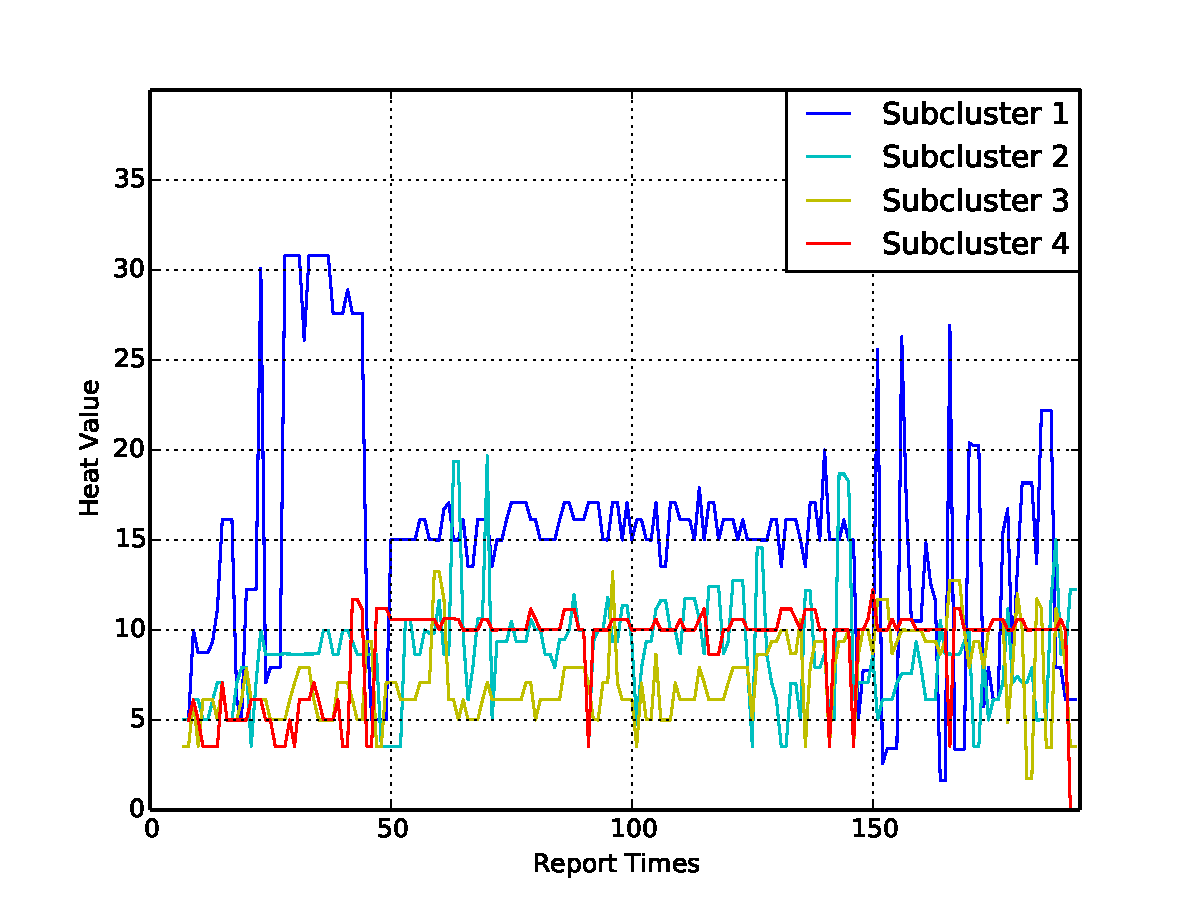
\includegraphics[width=10cm]{example/SingleMonitor.pdf}
    \bicaption[fig:heatdiffison0]{去掉全局热均衡的DOBBS子集群热度值}{去掉全局热均衡的DOBBS子集群热度值}{Fig}{Heat Value of Subcluster without Global Heat Balancing}
\end{figure}

\begin{figure}[!htp]
    \centering
    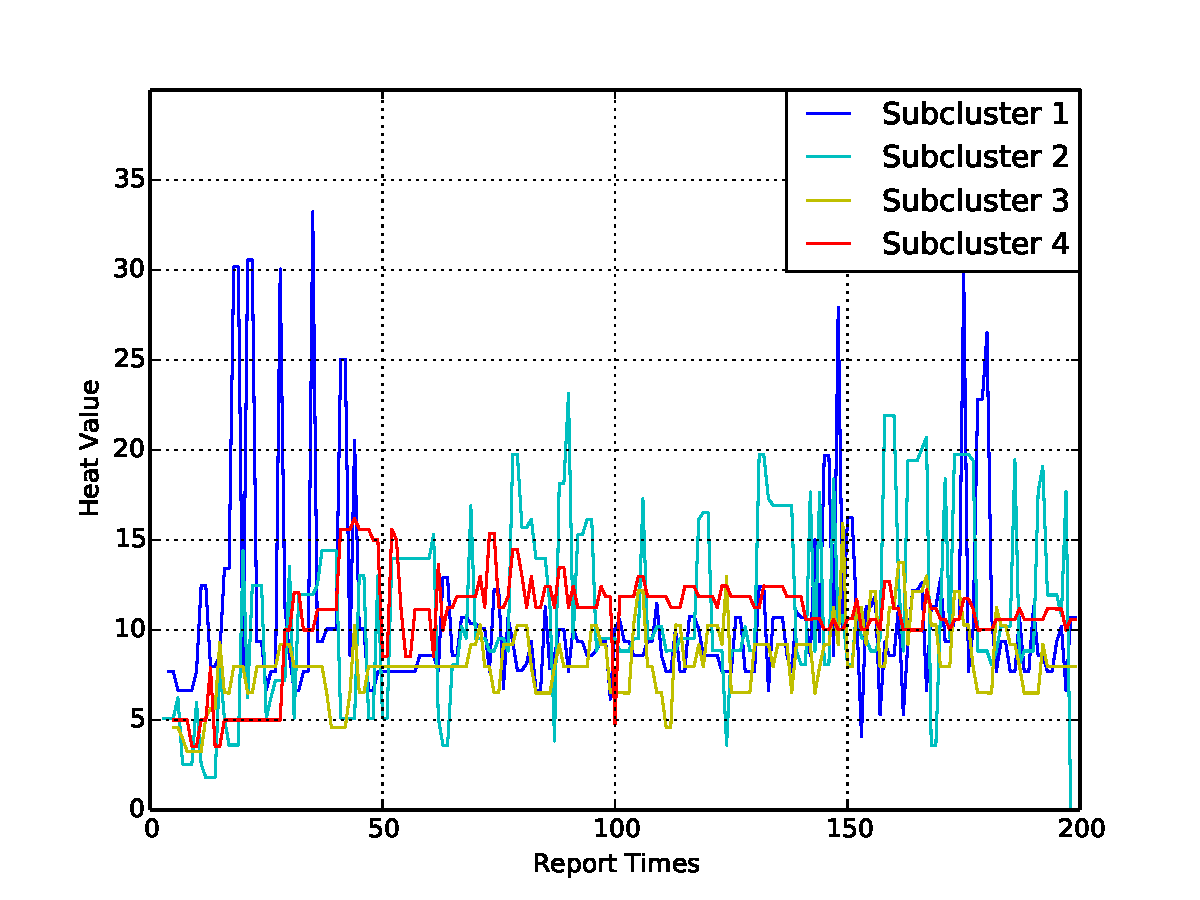
\includegraphics[width=10cm]{example/WithGHB.pdf}
    \bicaption[fig:heatdiffison0]{原始DOBBS的子集群热度值}{原始DOBBS的子集群热度值}{Fig}{Heat Value of Subcluster with Original DOBBS}
\end{figure}